\subsection{Approach}
\label{sys:appr}
We took a black-box approach to measure the prevalence of E-Mail Header Injection vulnerability on the World Wide Web. Black-box testing~\cite{wiki:Black-box_testing} is a way to examine the functionality of an application without looking at its source code.

As we did not have the source code for each of these websites, black-box testing was the ideal approach for this project. Black-box testing allows our system to detect E-Mail Header Injection vulnerabilities in any server-side language (not simply those we identified in Section~\ref{languages}). The overall architecture of our system is presented in Figure~\ref{fig:overall}. The components shown in Figure~\ref{fig:overall} can be more broadly categorized into different modules, as discussed in the following section.

\begin{figure*}
	\centering
	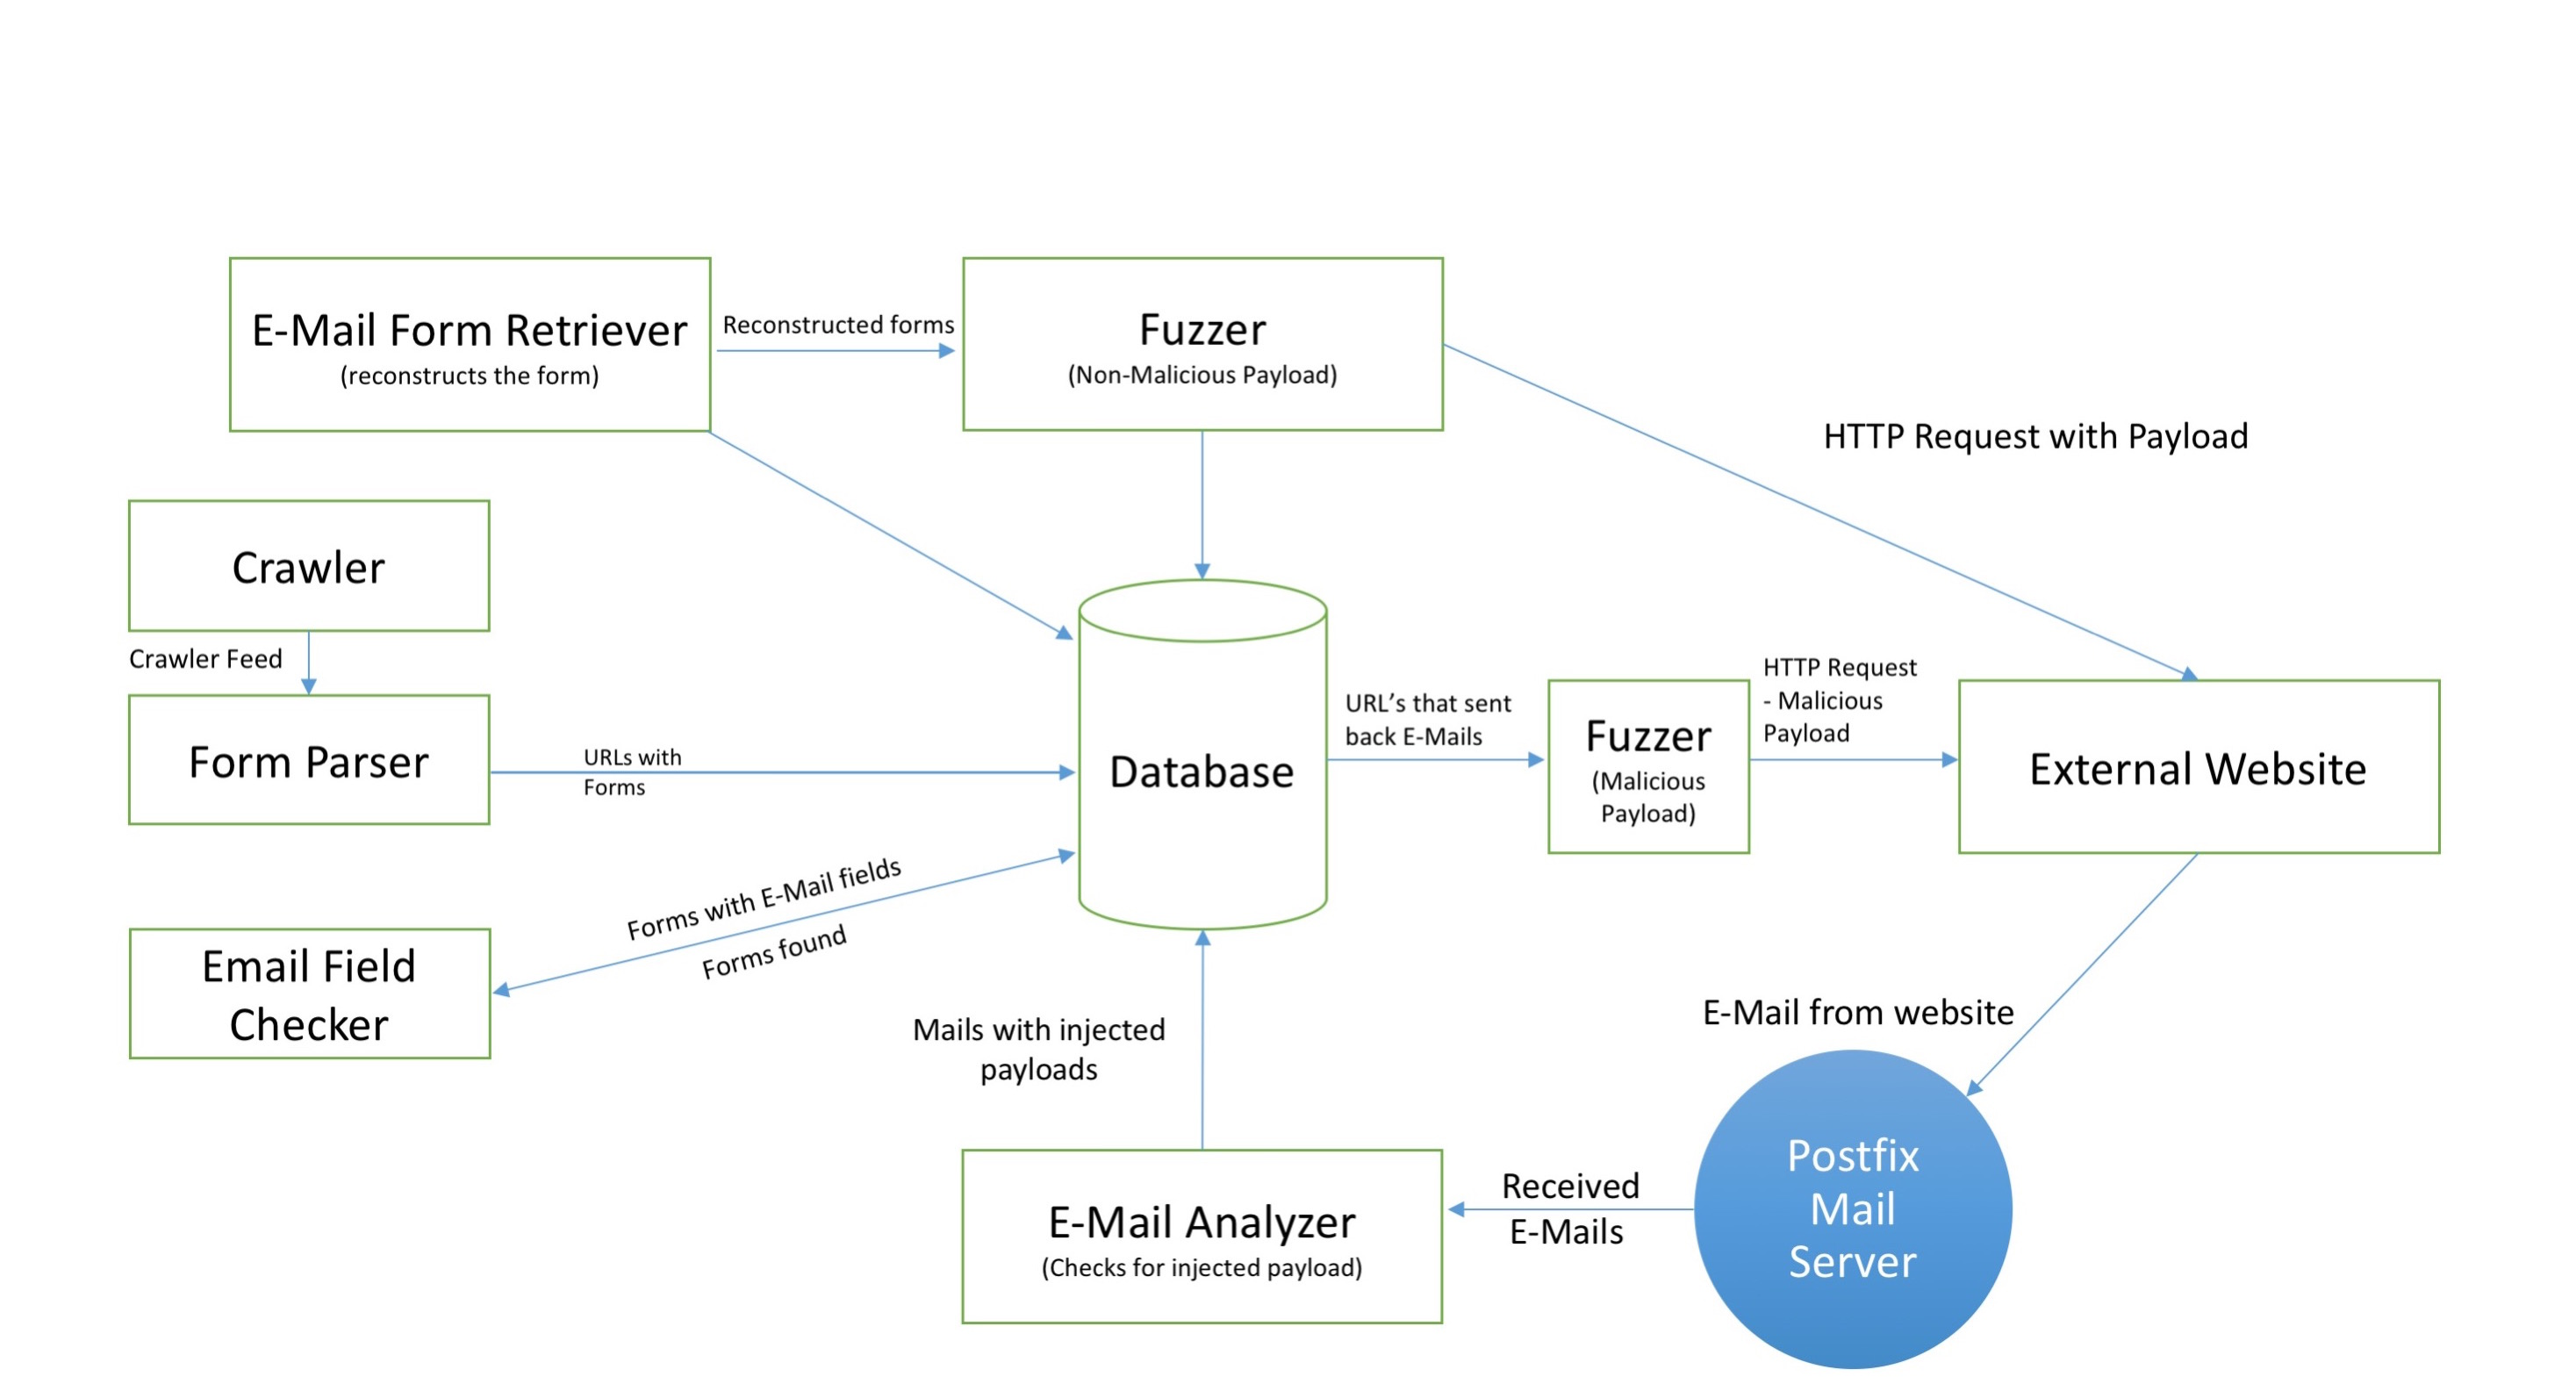
\includegraphics[width=14cm, height=7cm]{overall}
	\caption{Overall system architecture.}
	\label{fig:overall}
\end{figure*}
